\documentclass[12pt]{scrartcl}
\usepackage{comment} % enables the use of multi-line comments (\ifx \fi) 
\usepackage[english,german]{babel}
\usepackage{fancyhdr}
\usepackage{graphicx}
\usepackage{listings}
\usepackage[bottom=2cm]{geometry}
\usepackage{float}
\usepackage{wrapfig}
\usepackage{amsmath}
\usepackage[onehalfspacing]{setspace}
\usepackage{url}
\usepackage{tabularx}
\usepackage{caption}
\usepackage{eurosym}
\usepackage{subcaption}
\usepackage{pdfpages}
\usepackage{wrapfig}
\usepackage{color}
\usepackage{scrlayer-scrpage}%
\usepackage[T1]{fontenc}% wichtig für Trennung von Wörtern mit Umlauten
\usepackage{microtype}% verbesserter Randausgleich
\setlength{\headheight}{21.4pt}
\usepackage{apacite}
\usepackage{natbib}
\usepackage{eurosym}
\usepackage{amsmath}
\usepackage{algorithm}
\usepackage{algorithmicx}
\usepackage{eucal}% Special characters
\usepackage{amssymb}% math alphabet
\usepackage[noend]{algpseudocode}
\usepackage[utf8]{inputenc}

%%% Math %%%
\DeclareMathOperator{\EX}{\mathbb{E}}% expected value
\DeclareMathOperator*{\argmax}{argmax}

%%% Coding %%%
\colorlet{punct}{red!60!black}
\definecolor{background}{HTML}{EEEEEE}
\definecolor{delim}{RGB}{20,105,176}
\colorlet{numb}{magenta!60!black}

\lstdefinelanguage{json}{
    basicstyle=\normalfont\ttfamily,
    numbers=left,
    numberstyle=\scriptsize,
    stepnumber=1,
    numbersep=8pt,
    showstringspaces=false,
    breaklines=true,
    frame=lines,
    backgroundcolor=\color{background},
    literate=
     *{0}{{{\color{numb}0}}}{1}
      {1}{{{\color{numb}1}}}{1}
      {2}{{{\color{numb}2}}}{1}
      {3}{{{\color{numb}3}}}{1}
      {4}{{{\color{numb}4}}}{1}
      {5}{{{\color{numb}5}}}{1}
      {6}{{{\color{numb}6}}}{1}
      {7}{{{\color{numb}7}}}{1}
      {8}{{{\color{numb}8}}}{1}
      {9}{{{\color{numb}9}}}{1}
      {:}{{{\color{punct}{:}}}}{1}
      {,}{{{\color{punct}{,}}}}{1}
      {\{}{{{\color{delim}{\{}}}}{1}
      {\}}{{{\color{delim}{\}}}}}{1}
      {[}{{{\color{delim}{[}}}}{1}
      {]}{{{\color{delim}{]}}}}{1},
}

%Pseudo-code indent
\algdef{SE}[SUBALG]{Indent}{EndIndent}{}{\algorithmicend\ }%
\algtext*{Indent}
\algtext*{EndIndent}

%Pseudo-code indent
\algdef{SE}[SUBALG]{Indent}{EndIndent}{}{\algorithmicend\ }%
\algtext*{Indent}
\algtext*{EndIndent}


%%%% footer and header %%%%

\setlength{\parindent}{0em}
\setlength{\parskip}{2mm}

\pagestyle{scrheadings}%  S
\clearscrheadfoot% 
\setheadwidth{text}%
\automark{section}% 
\ihead{\textbf{\pagemark}}
\renewcommand{\sectionmark}[1]{\markright{\ #1}} 
\ohead{\rightmark}
\setheadsepline{0.5pt}
\renewcommand{\labelenumii}{\theenumii}
\renewcommand{\theenumii}{\theenumi.\arabic{enumii}.}
%%%% \footer and header %%%%

% Funktion, um besser Anführungszeichen zu setzen.
% Einfach \anf{Wort oder Text}
\newcommand{\anf}[1]{
\glqq #1\grqq{}
}

\begin{document}

\begin{titlepage}
\newgeometry{top=1cm, left=3cm, right=3cm}
\begin{tabular}{lcr}
  \hspace{10cm} &
  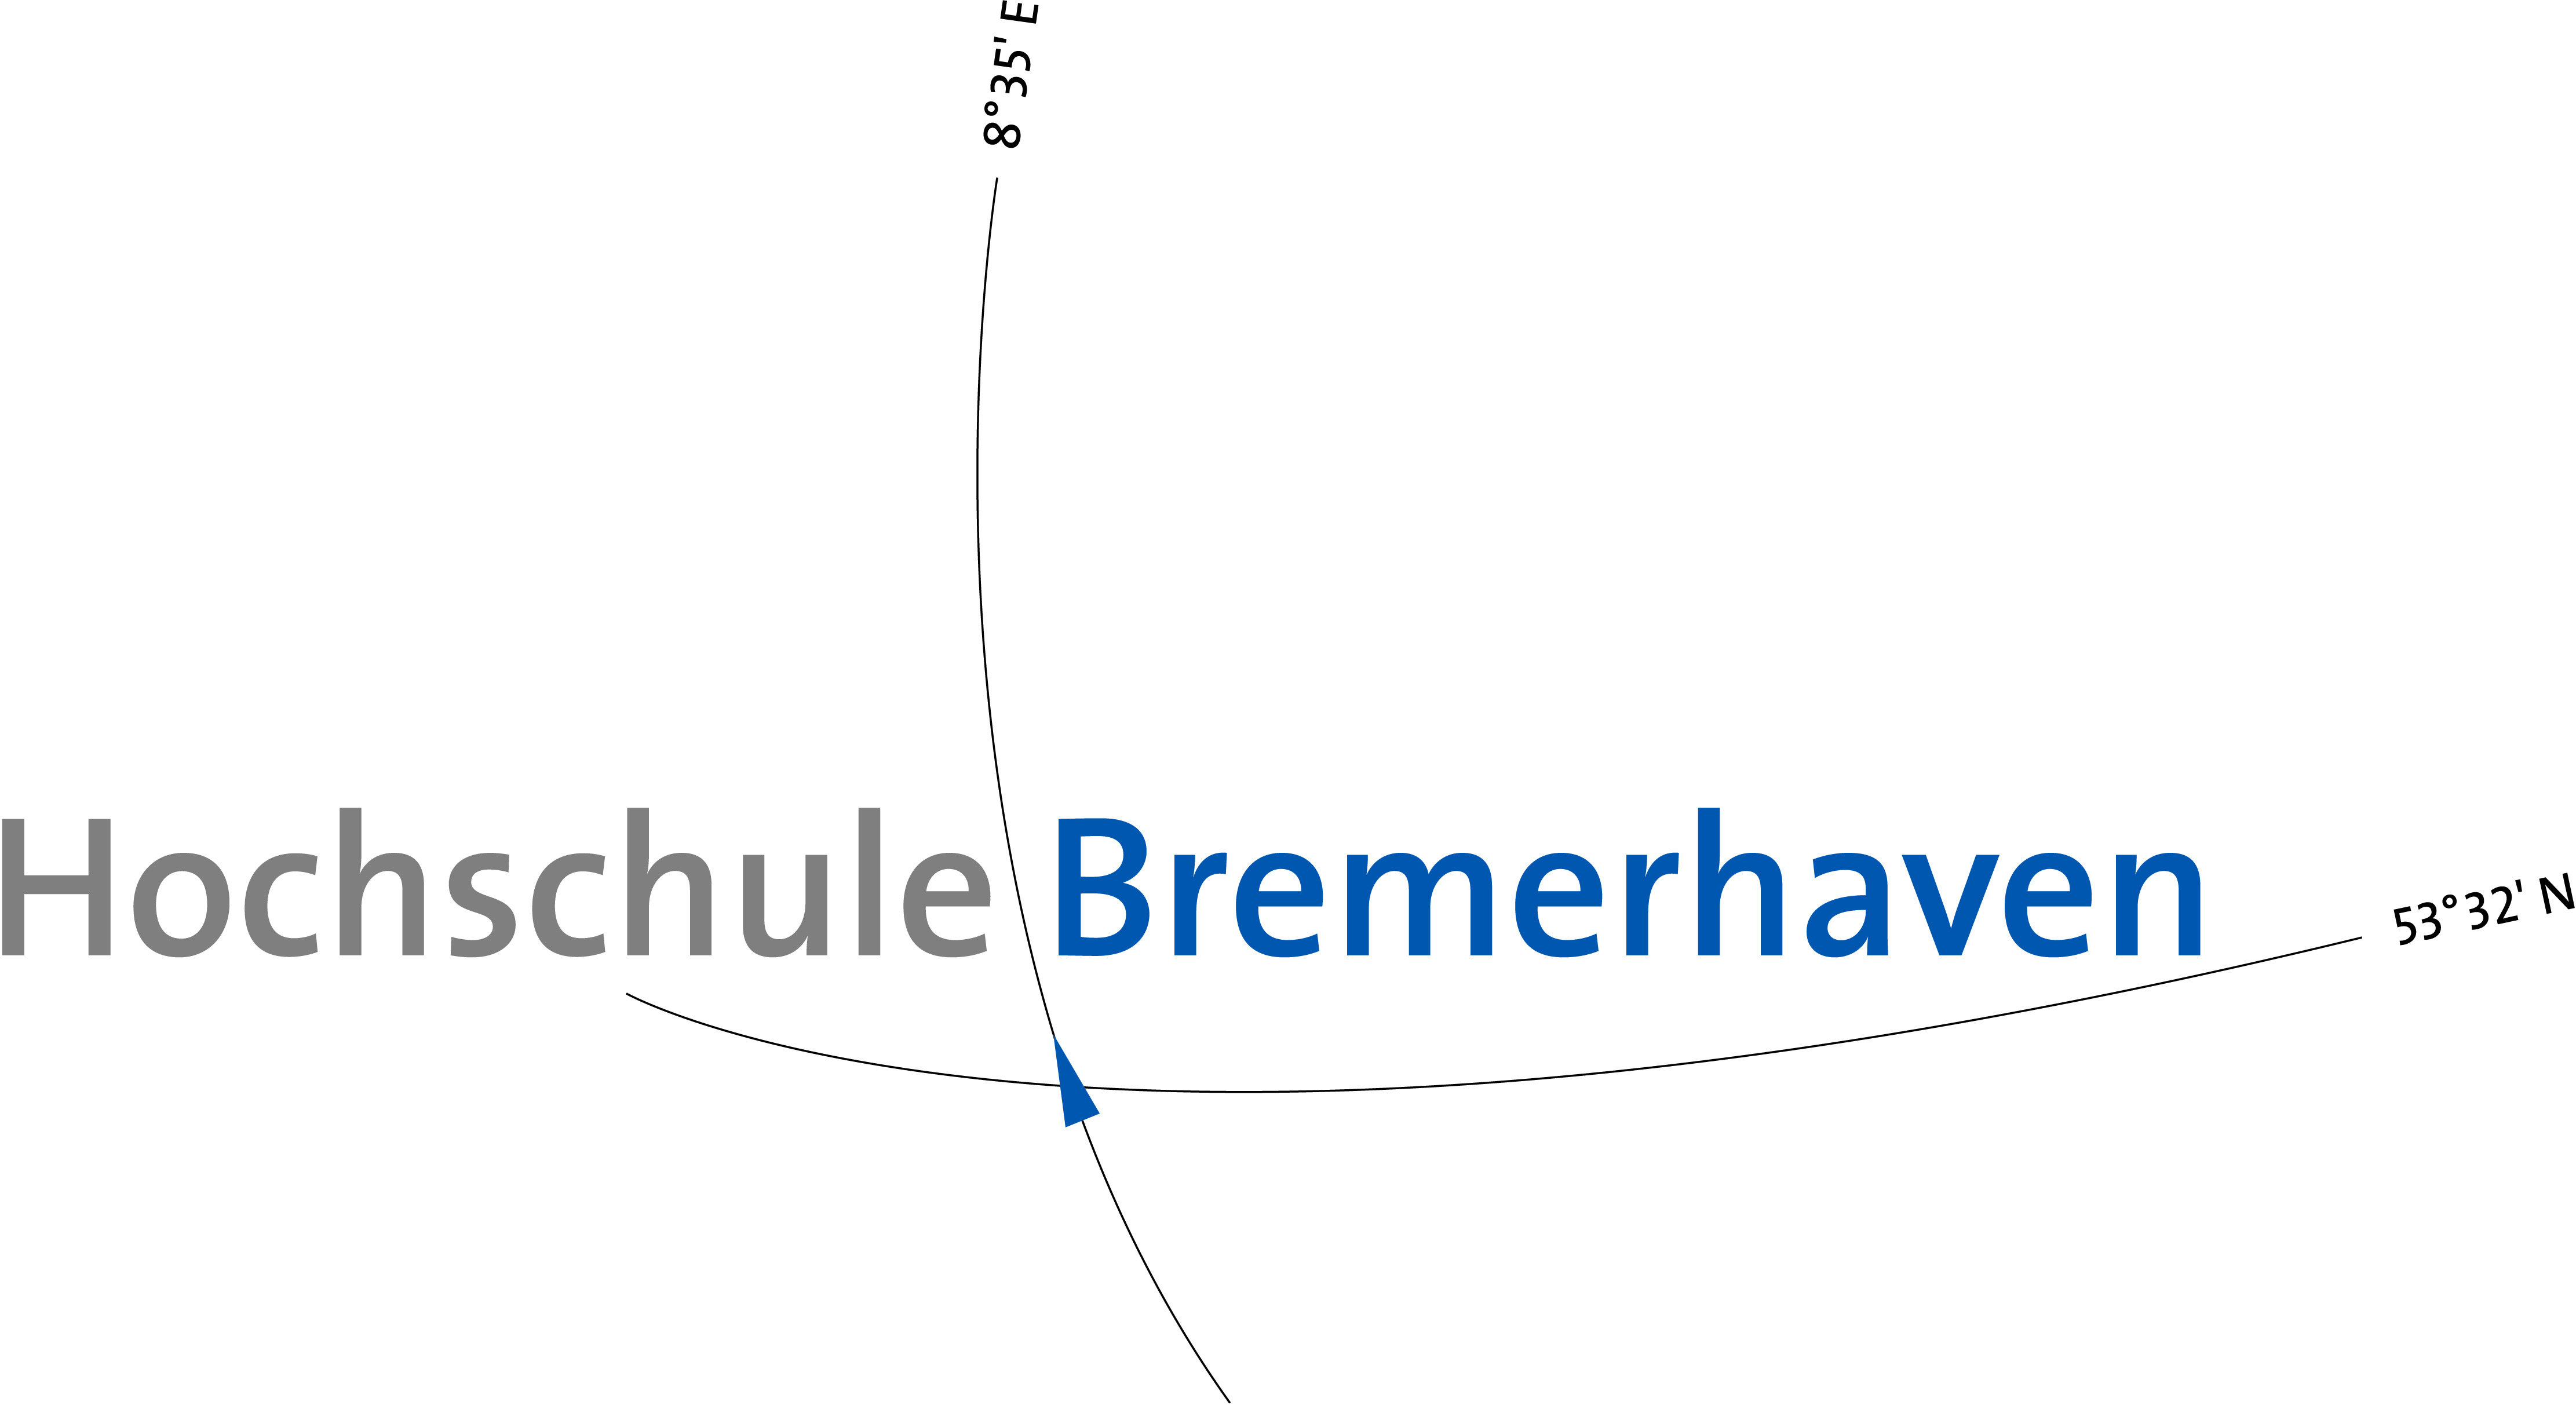
\includegraphics[width=170px]{images/hb_logo_2c.jpg}
  \vspace{1cm}
\end{tabular}
	\centering	
	\vspace{1cm}
	{\scshape\Large Small heading \par}
	\vspace{1.5cm}
	{\huge\bfseries Major Heading of the Project\par}
    \vspace{2cm}
    {\Large\itshape 
        Italic block with detailed information about the project that should generally not exceed one sentence
        	\par}
	\vfill
	\begin{tabularx}{\textwidth}{lX}
		Autoren: & Name One (StudentID), Name Two (StudentID) \\
		Prüfer: & Prof. Dr. Ing. Nice Prof, Prof. Dr. Bad Prof  \\
		        
	\end{tabularx}  
    \vfill

% Bottom of the page with current date
	{\large \today \par}       
\end{titlepage}
\restoregeometry

% Abstrakt bzw. Zusammenfassung ('*' macht, dass es nicht im Inhaltsverzeichnis auftaucht, aber trotzdem den Stil einer Überschrift hat
\section*{Abstract}
This is the abstract. Should not exceed one page.
\newpage
% Inhaltsverzeichnis
\tableofcontents
\newpage
% Abbildungsverzeichnis
\listoffigures
\newpage
\noindent

\section{Einleitung} \label{sec:einleitung}
Lorem ipsum dolor sit amet, consetetur sadipscing elitr, sed diam nonumy eirmod tempor invidunt ut labore et dolore magna aliquyam erat, sed diam voluptua. At vero eos et accusam et justo duo dolores et ea rebum. Stet clita kasd gubergren, no sea takimata sanctus est Lorem ipsum dolor sit amet.
    \subsection{Zitieren}
    Wie man zitiert. Für indirekte Zitate setzt man am Ende ganz einfach den Snippet: \begin{verbatim}
\cite[]{anderie2018gamification}
\end{verbatim}
Selbst wenn keine Seitenanzahlen angegeben werden, müssen die einfachen Klammern nach dem cite-Befehl gesetzt werden, weil ein zusätzliches Package (natbib) eingebunden ist, welches passive Autorenzitierung erlaubt \cite[]{anderie2018gamification}. Für das Einbinden der Seitenanzahl, kann einfach in die eckigen Klammern geschrieben werden, z.B. \anf{S.\textasciitilde10f.}, dabei sorgt die Tilde für einen gleichbleibenden Abstand des Leerzeichens \cite[S.~10f.]{anderie2018gamification}. 
\par 
Wird über mehrere Sätze hinweg zitiert kann ein Trick angewendet werden. Dabei werden die Autoren direkt in die Sätze mit eingebunden und deren Aussagen über mehrere Sätze hin verknüpft. Beispiel:\par 
\cite{Stef12} beschreiben in ihrer Arbeit drei grundsätzliche Konzepte, die allesamt eine Rolle in der Gamifizierung spielen. Die Autoren weisen darauf hin, dass vor allem das Konzept A die größte Bedeutung hat. Dennoch sind sie der Meinung, dass es in der nahen Zukunft zu einer großen Veränderung kommen wird, die sich hauptsächlich durch Grund B begründet lässt (S.~25ff.).
\par 
Diese Art der Zitierung kann erreicht werden, indem die eckigen Klammern entfernt werden:
\begin{verbatim}
\cite{Stef12}
\end{verbatim}
Die referenzierten Seiten werden einfach per Hand am Ende des Absatzes hinzugefügt.
\par
Bilder und Kapitel referenziert man ganz einfach mit:
\begin{verbatim}
\ref{fig:hslogoRight} 
\ref{sec:mathe}

Sind die Bezeichnungen der Label.
\label{fig:hslogoRight}
\end{verbatim}
In Abbildung \ref{fig:hslogoRight} erkennt man...
\par 
Im Kapitel \ref{sec:sonstiges} wird beschrieben, dass
    \subsection{Bilder}
    \begin{verbatim}
\begin{figure}[H]
    \centering
    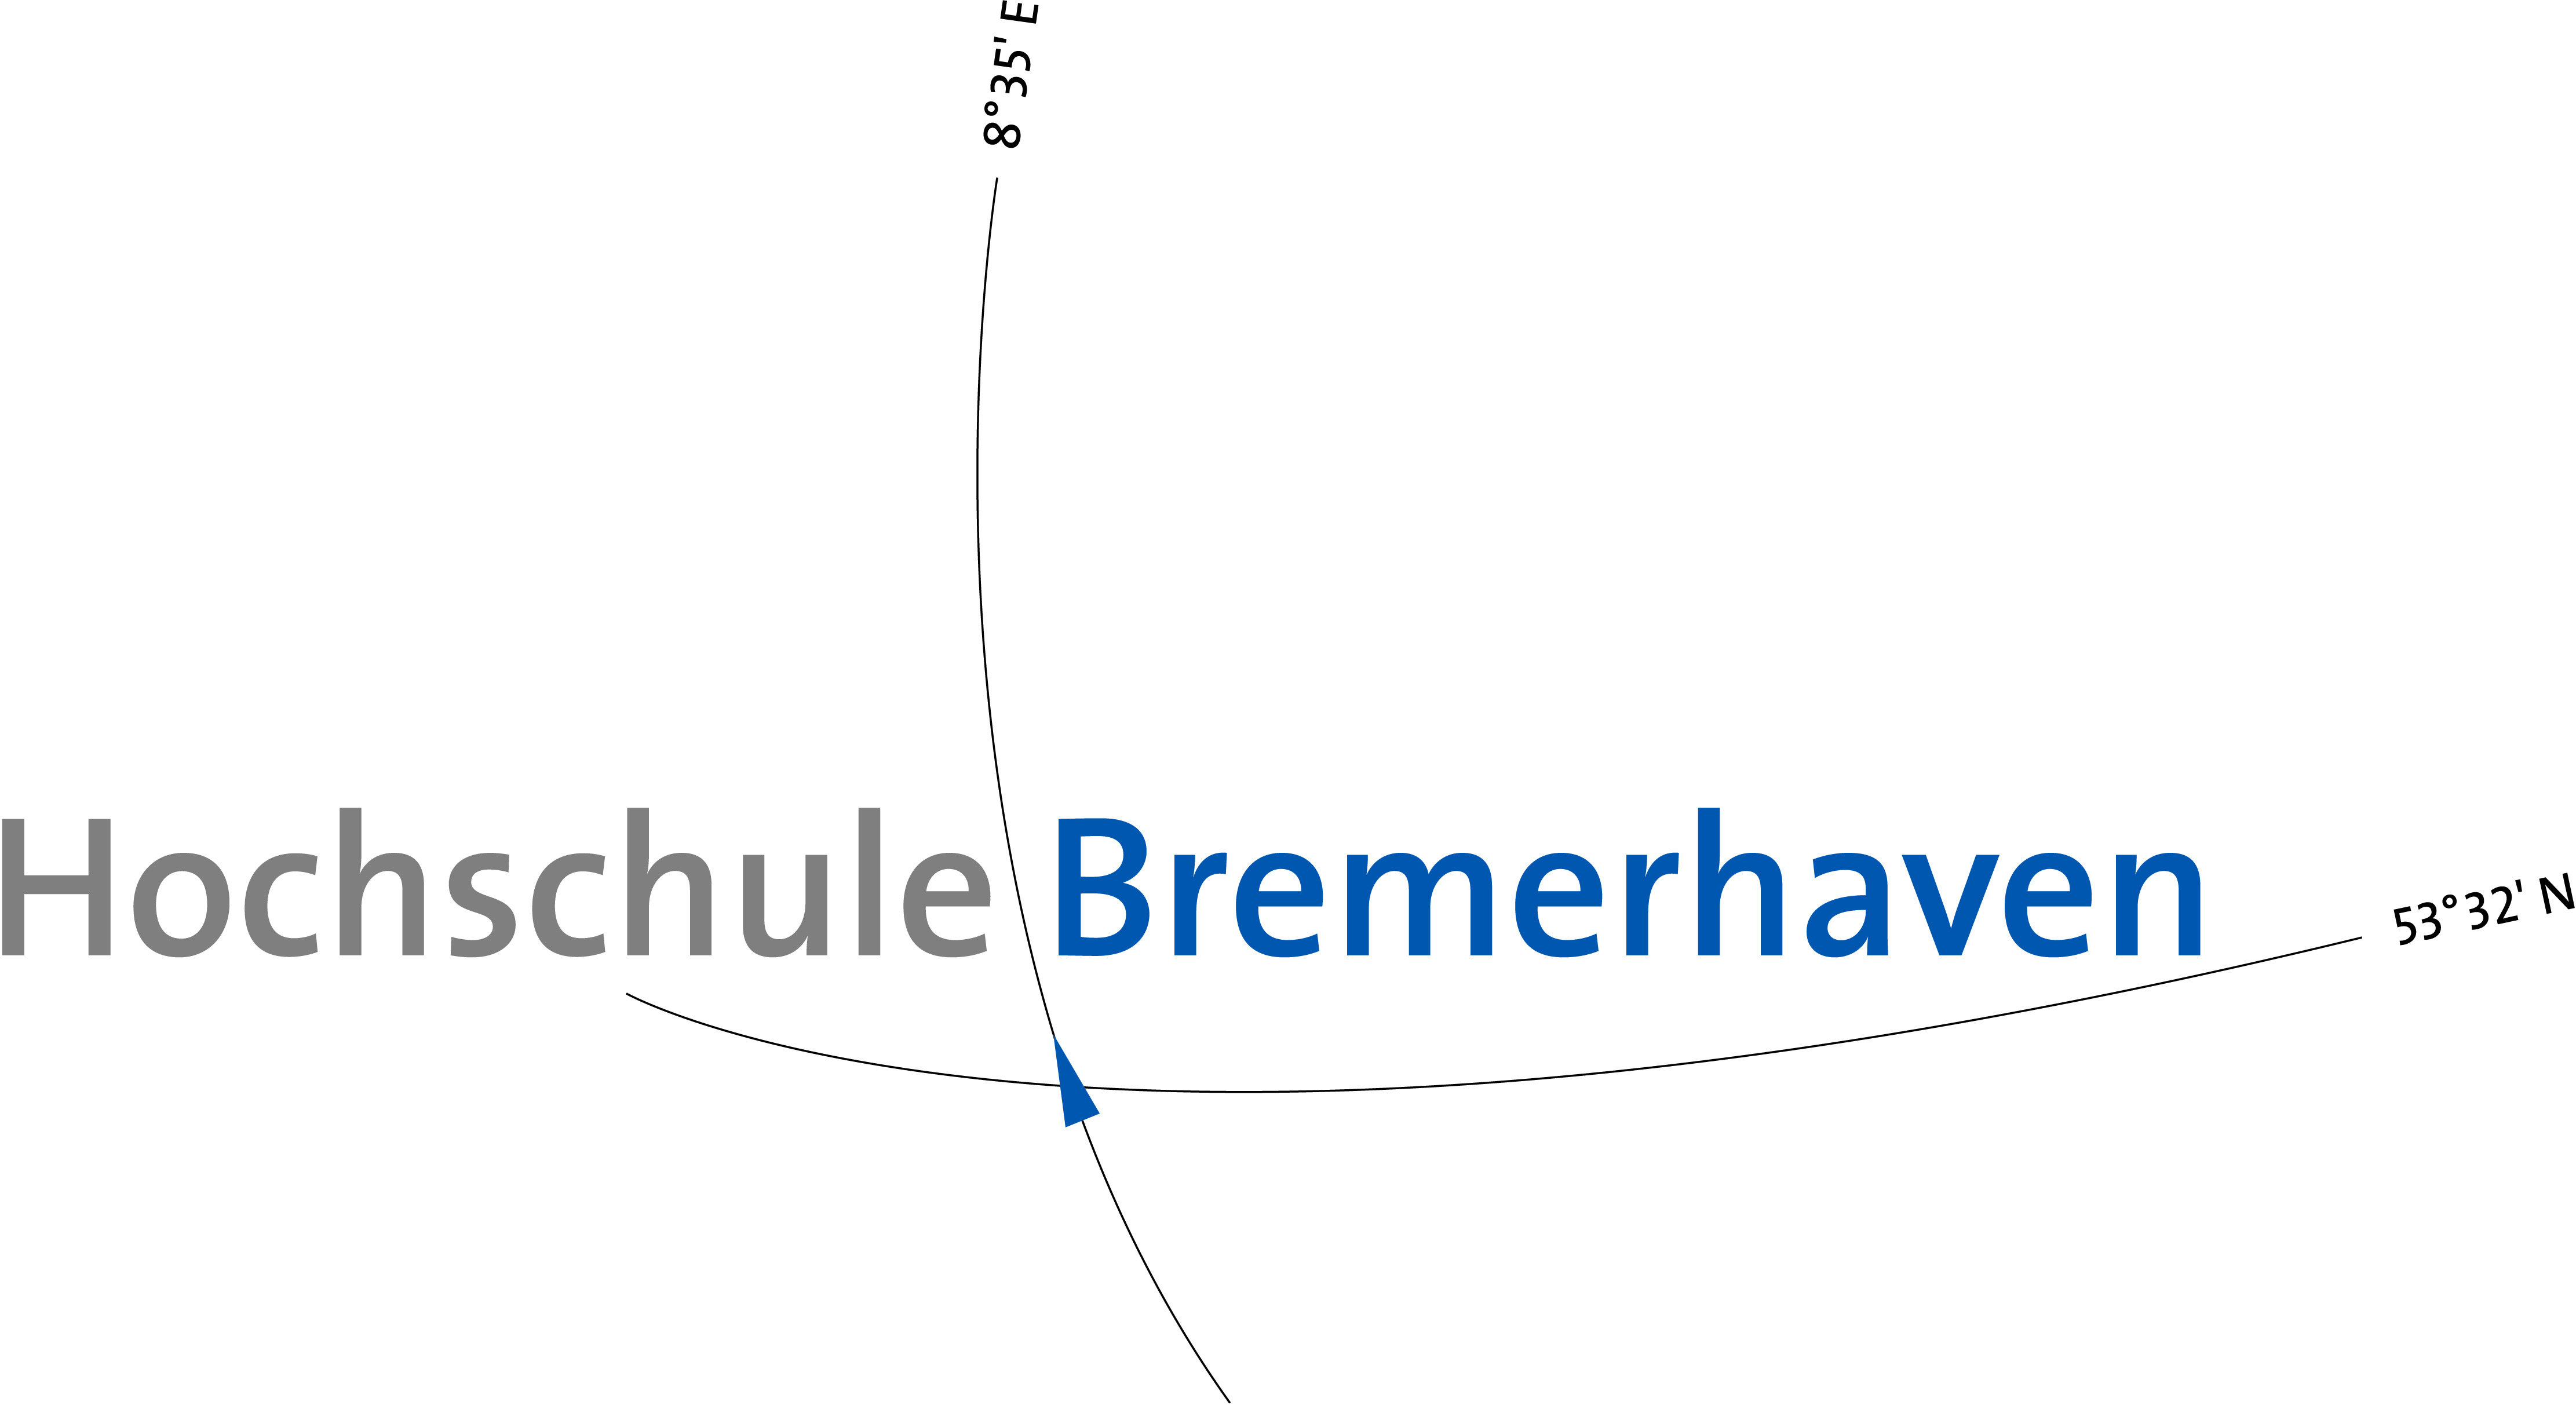
\includegraphics[width=0.7\textwidth]{images/hb_logo_2c.jpg}
    \captionof{figure}{Hochschullogo}
    \label{fig:hslogo}
\end{figure}
\end{verbatim}
\begin{figure}[H]
    \centering
    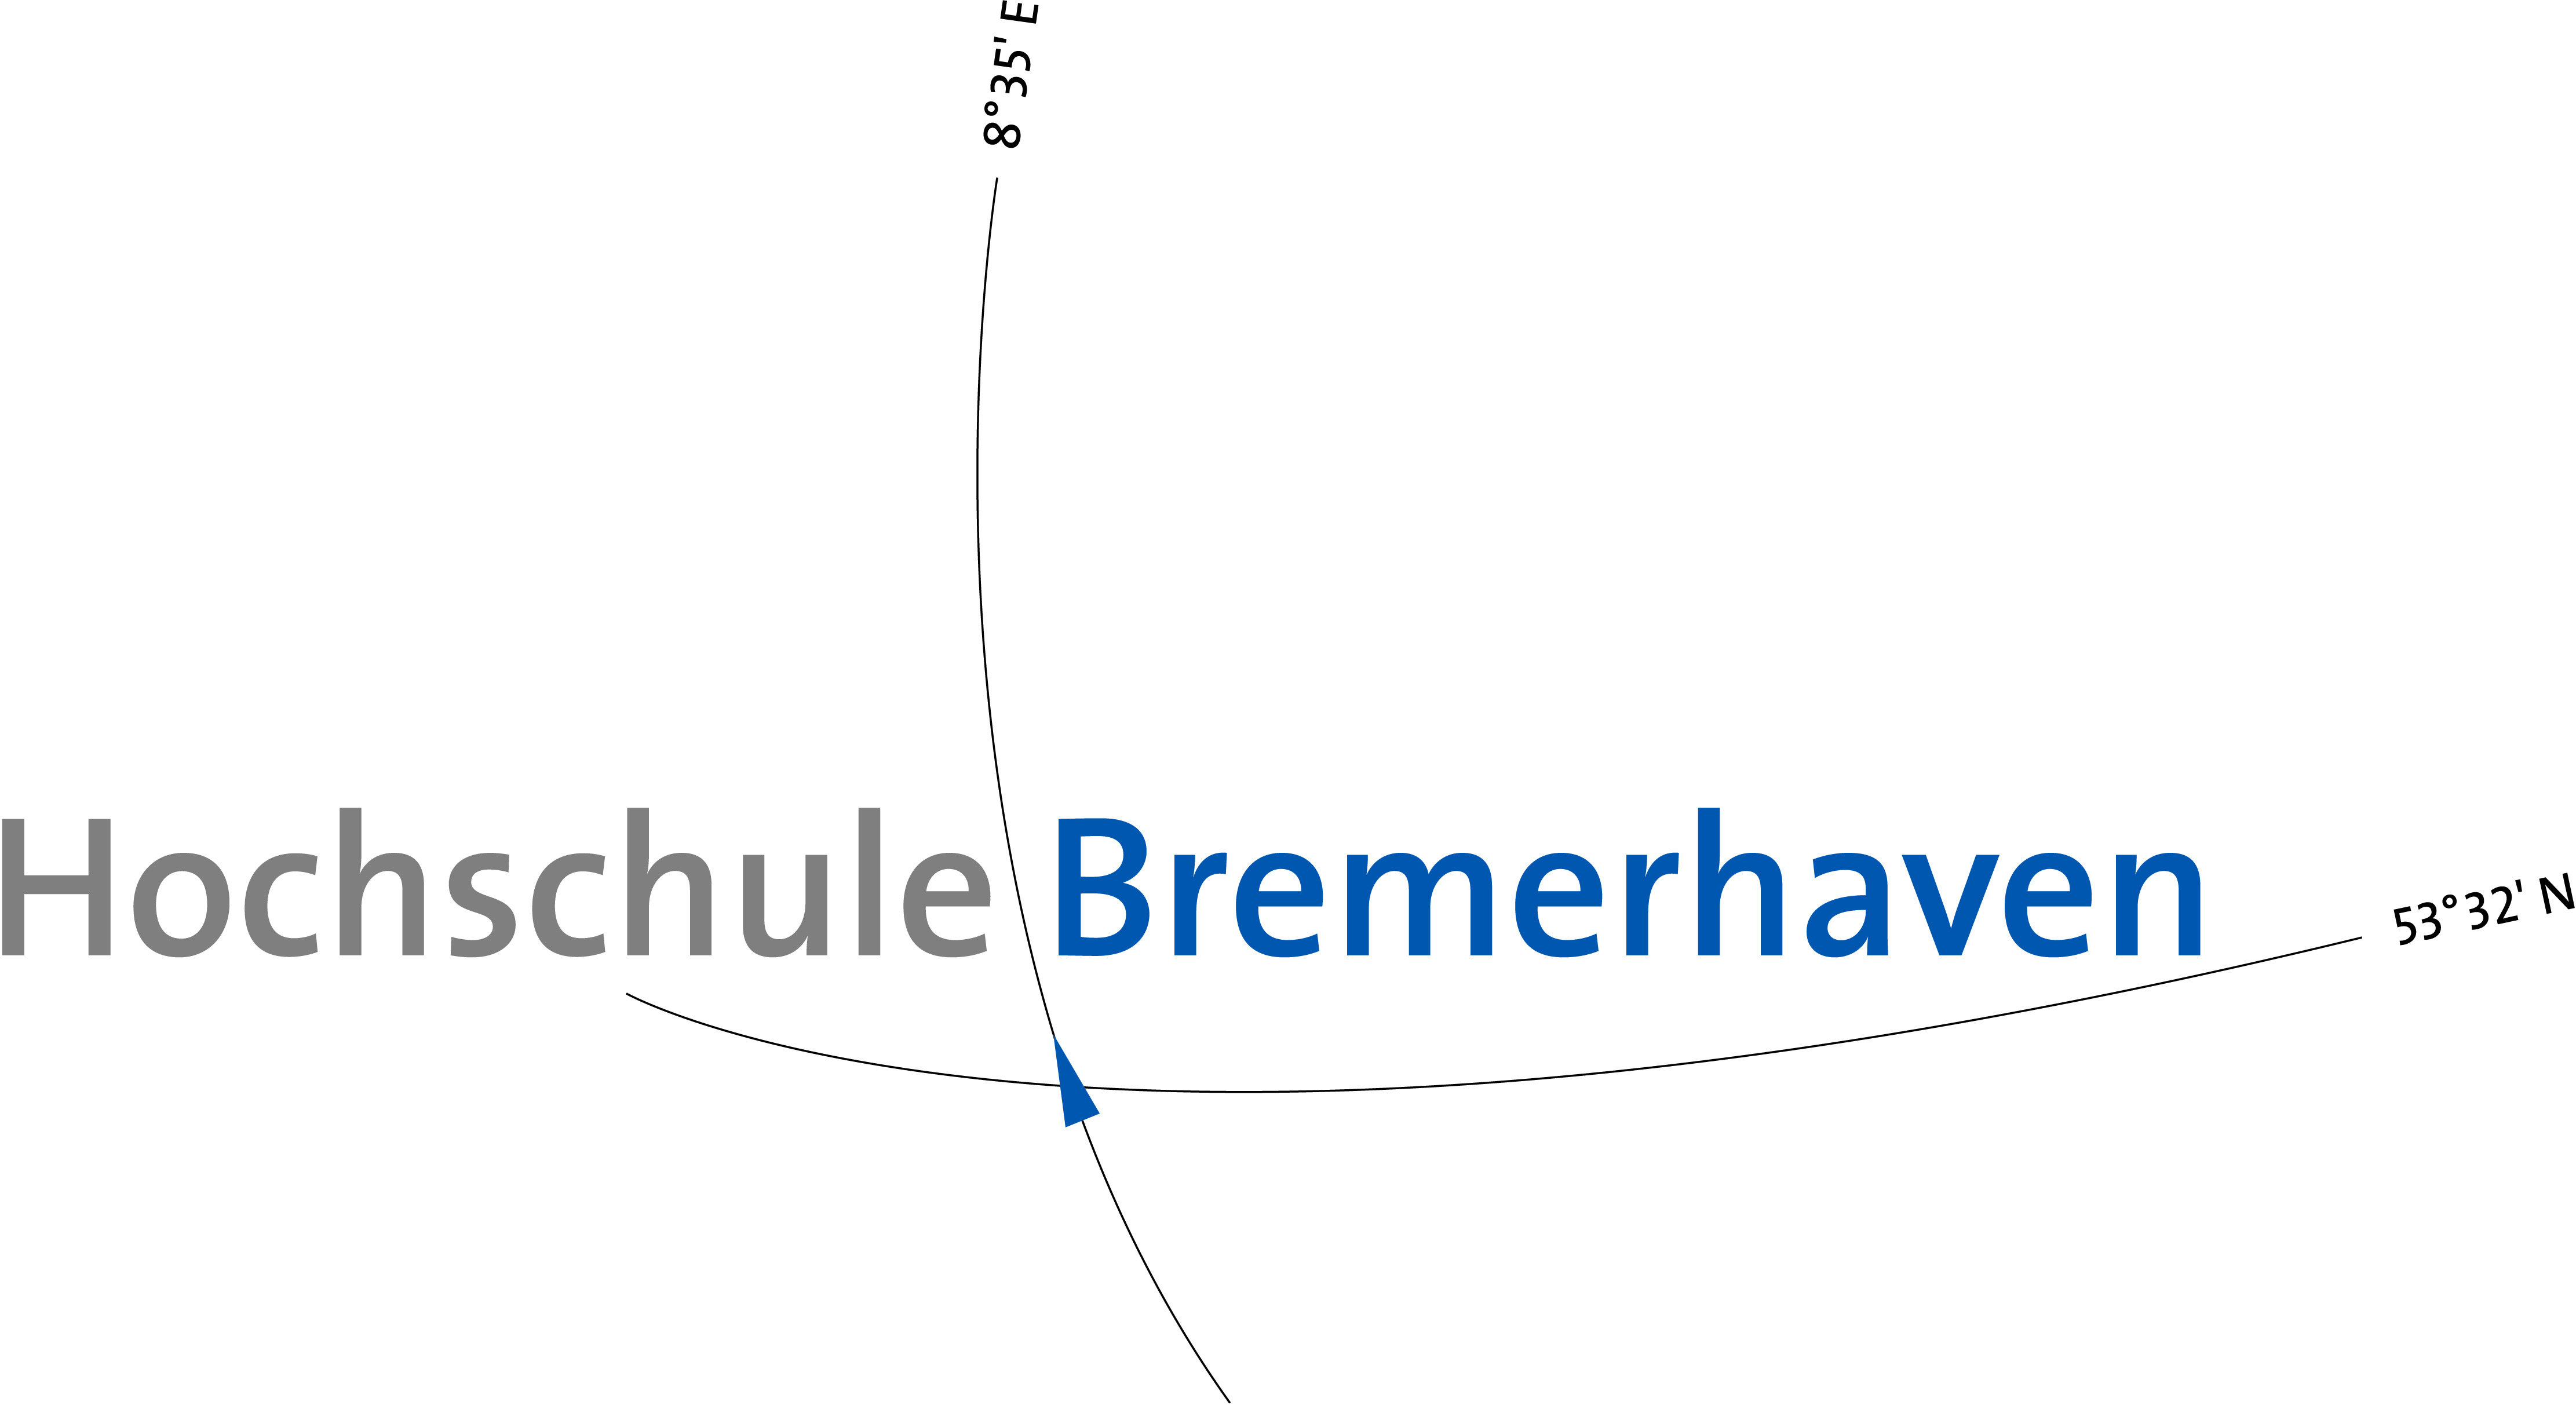
\includegraphics[width=0.7\textwidth]{images/hb_logo_2c.jpg}
    \captionof{figure}{Hochschullogo}
    \label{fig:hslogo}
\end{figure}

\begin{verbatim}
\begin{figure}[H]
    \centering
    \begin{minipage}{.47\textwidth}
      \centering
      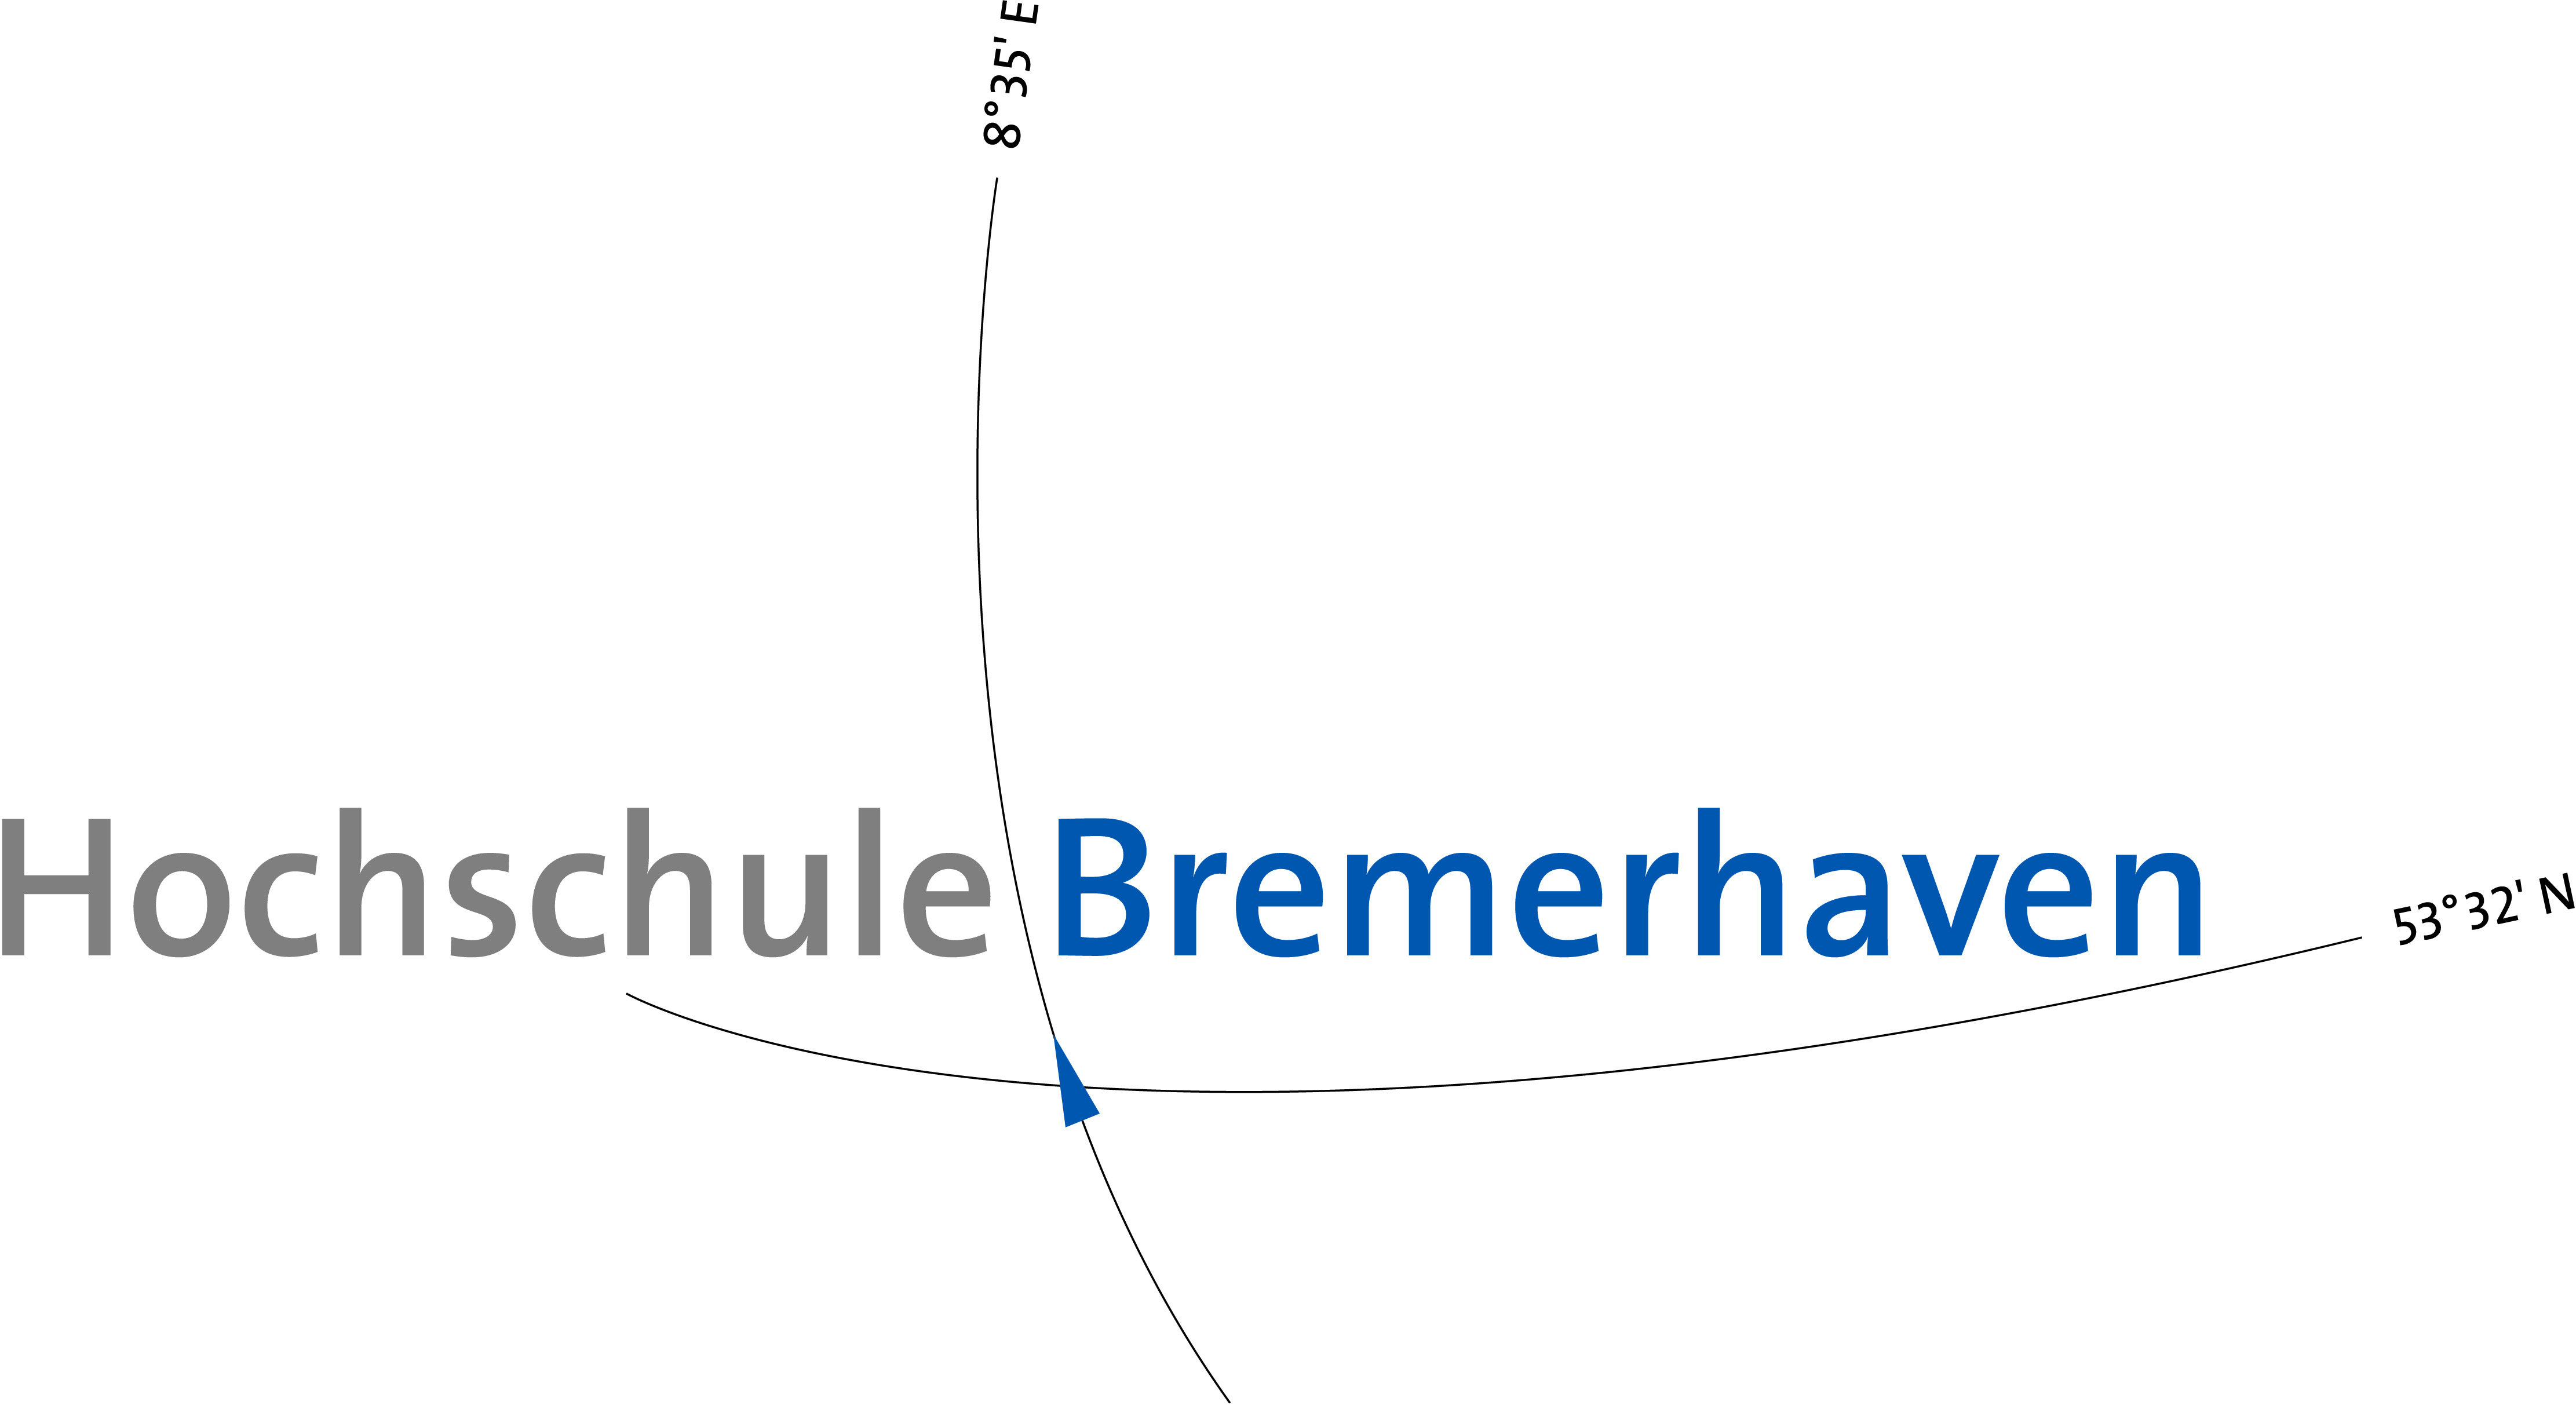
\includegraphics[width=\textwidth]{images/hb_logo_2c.jpg}
      \captionof{figure}{links}
      \label{fig:hslogoLeft}
    \end{minipage}
    \hspace{.05\textwidth}%
    \begin{minipage}{.47\textwidth}
        \centering
        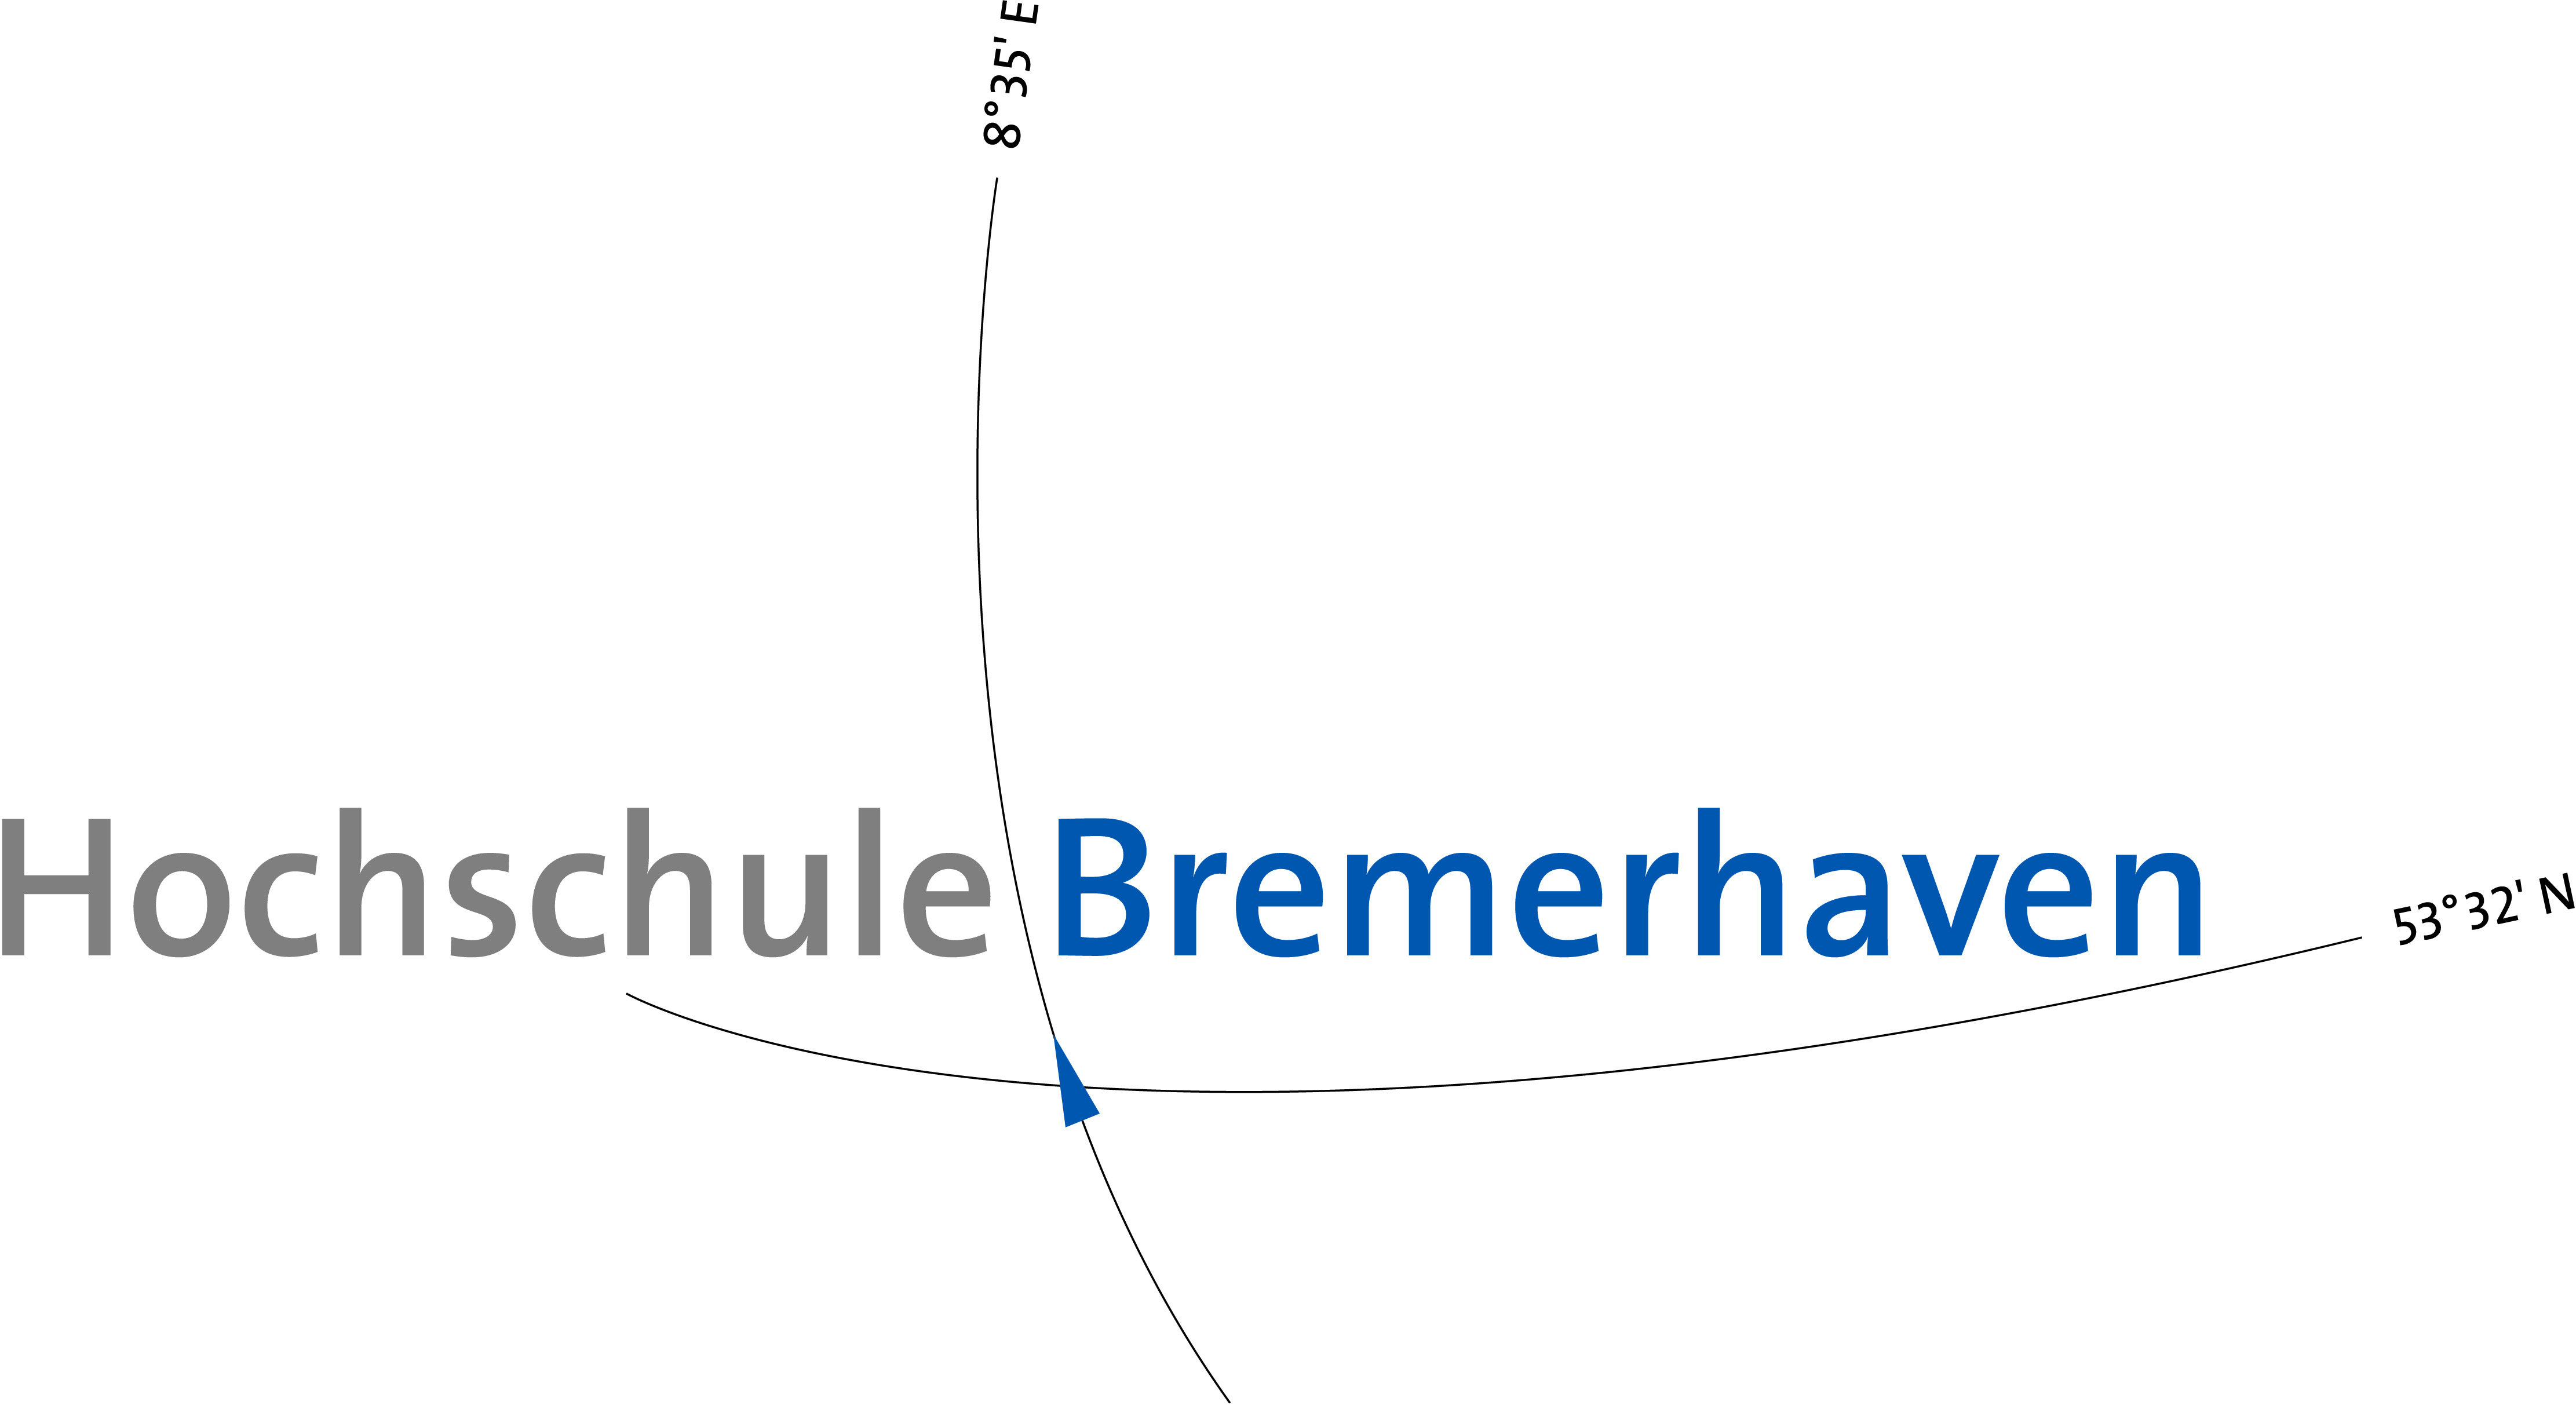
\includegraphics[width=\textwidth]{images/hb_logo_2c.jpg}
        \captionof{figure}{rechts}
        \label{fig:hslogoRight}
      \end{minipage}
\end{figure}
\end{verbatim}
\begin{figure}[H]
    \centering
    \begin{minipage}{.47\textwidth}
      \centering
      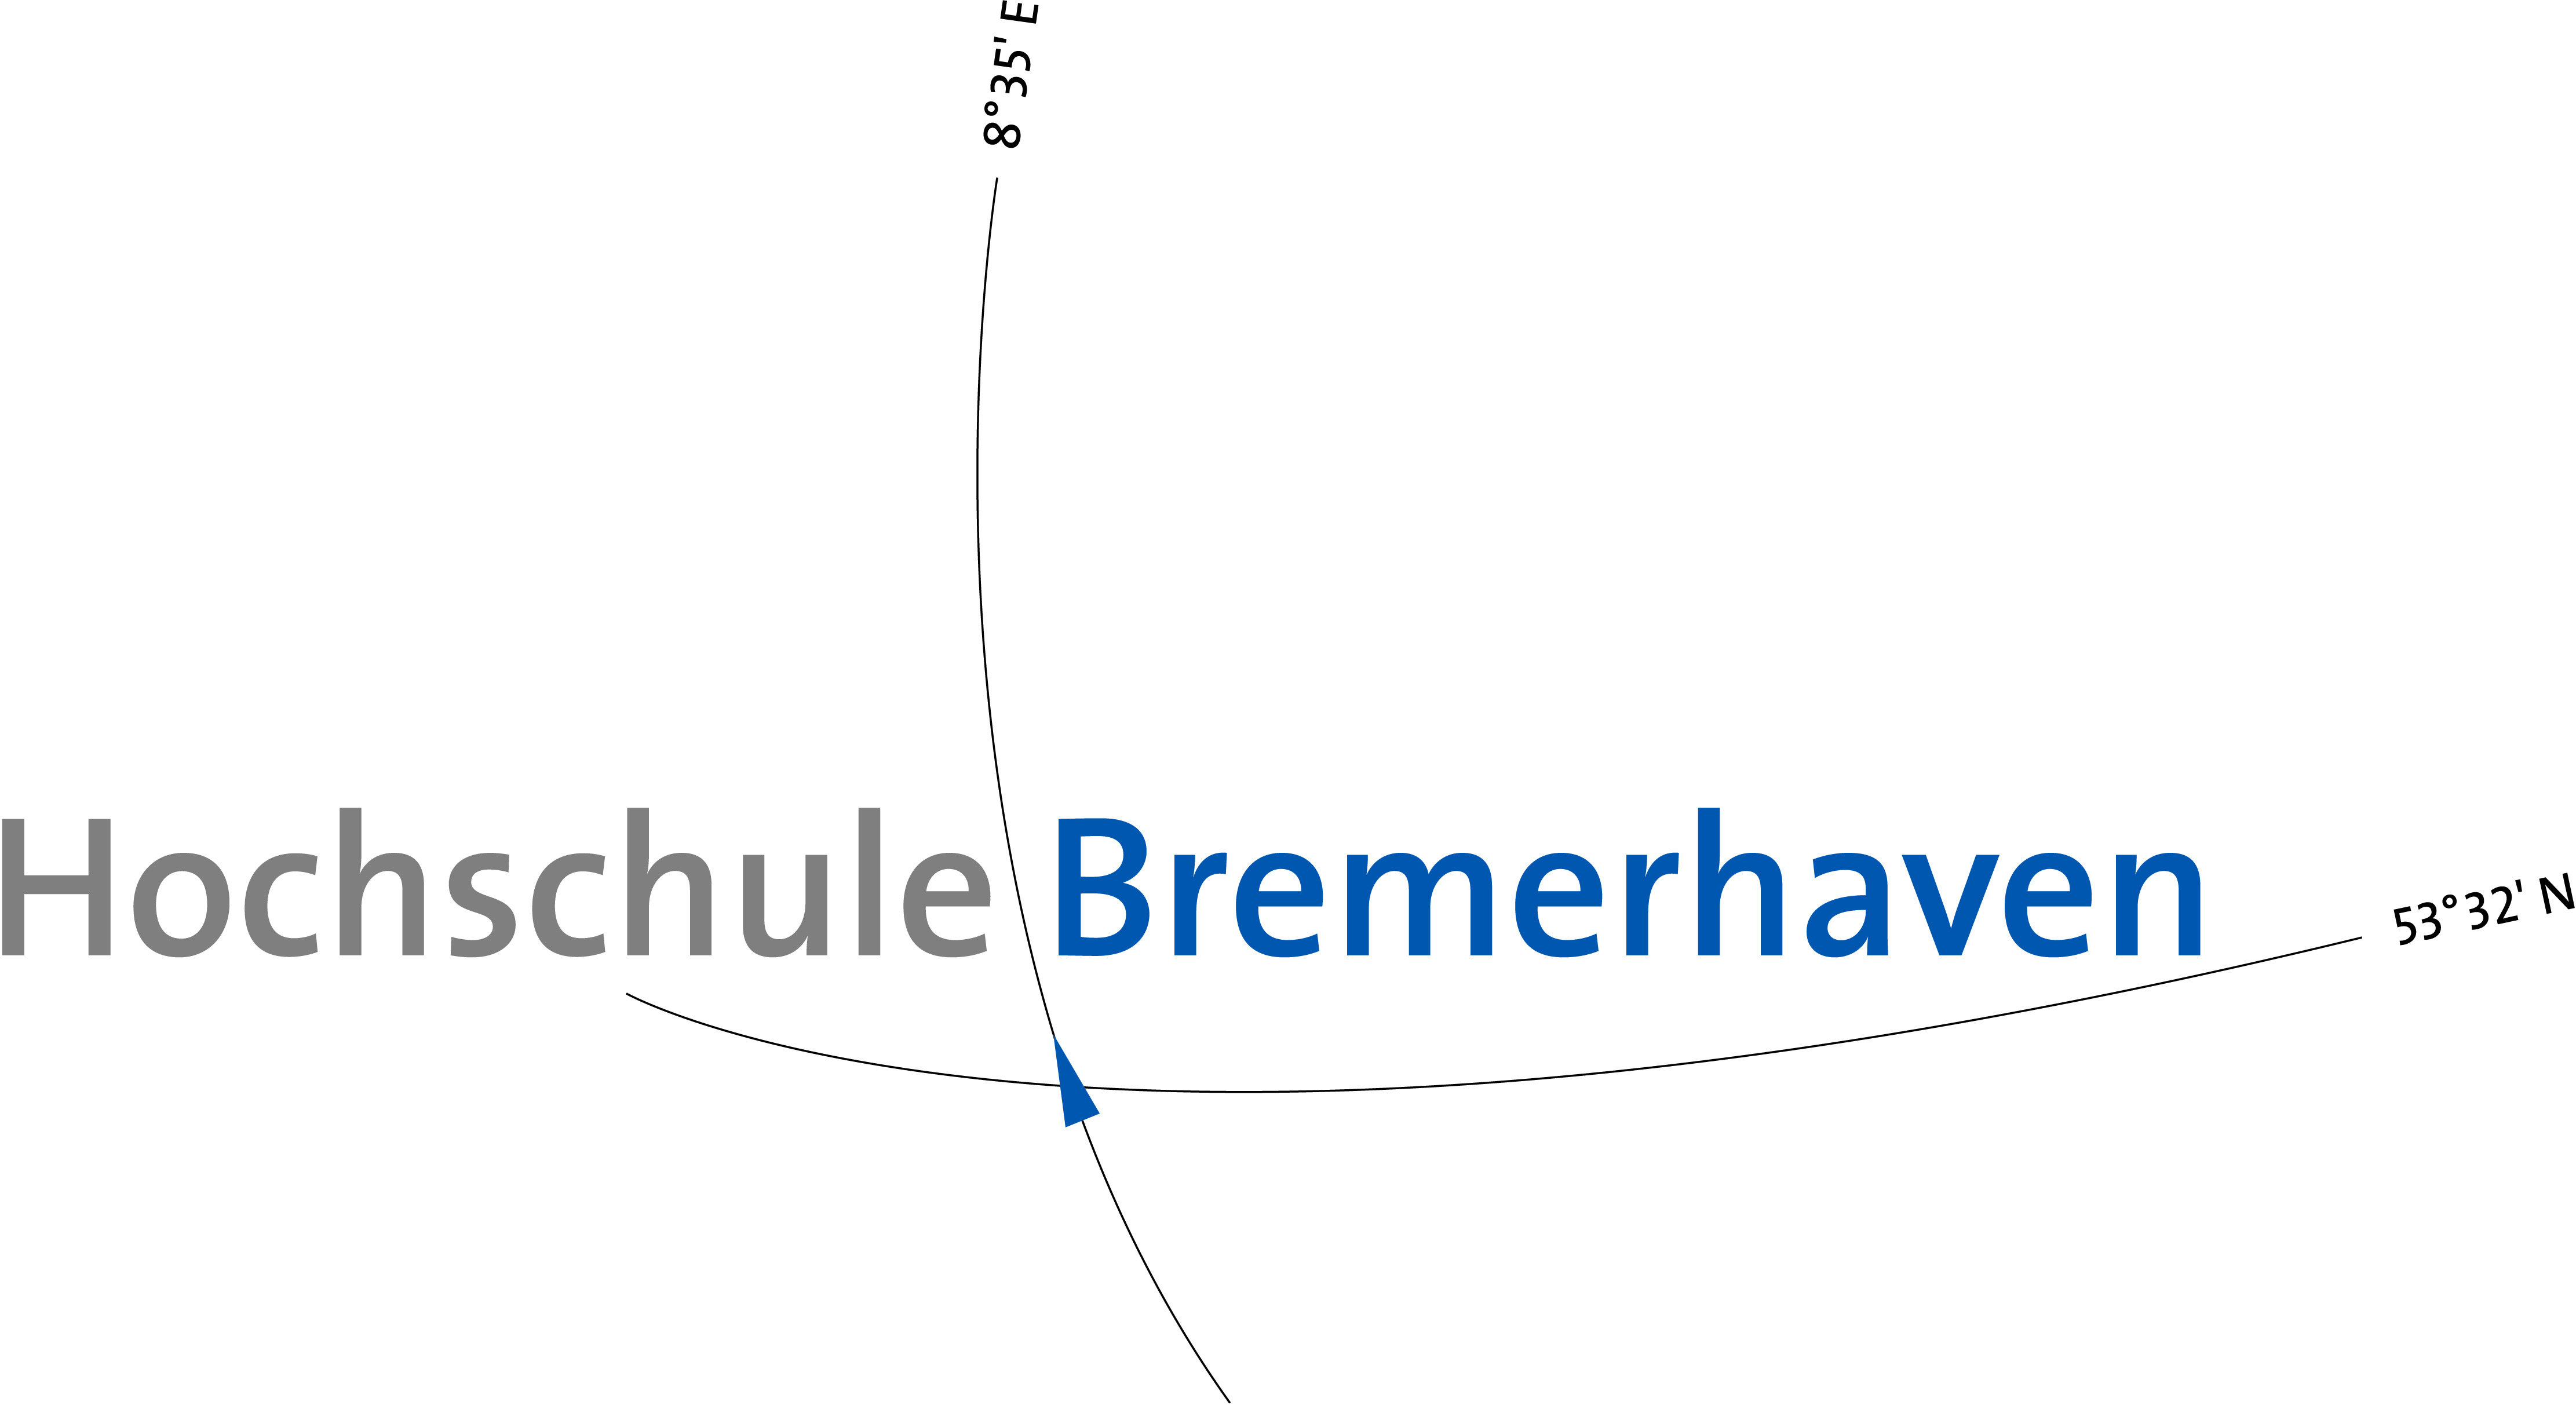
\includegraphics[width=\textwidth]{images/hb_logo_2c.jpg}
      \captionof{figure}{links}
      \label{fig:hslogoLeft}
    \end{minipage}
    \hspace{.05\textwidth}%
    \begin{minipage}{.47\textwidth}
        \centering
        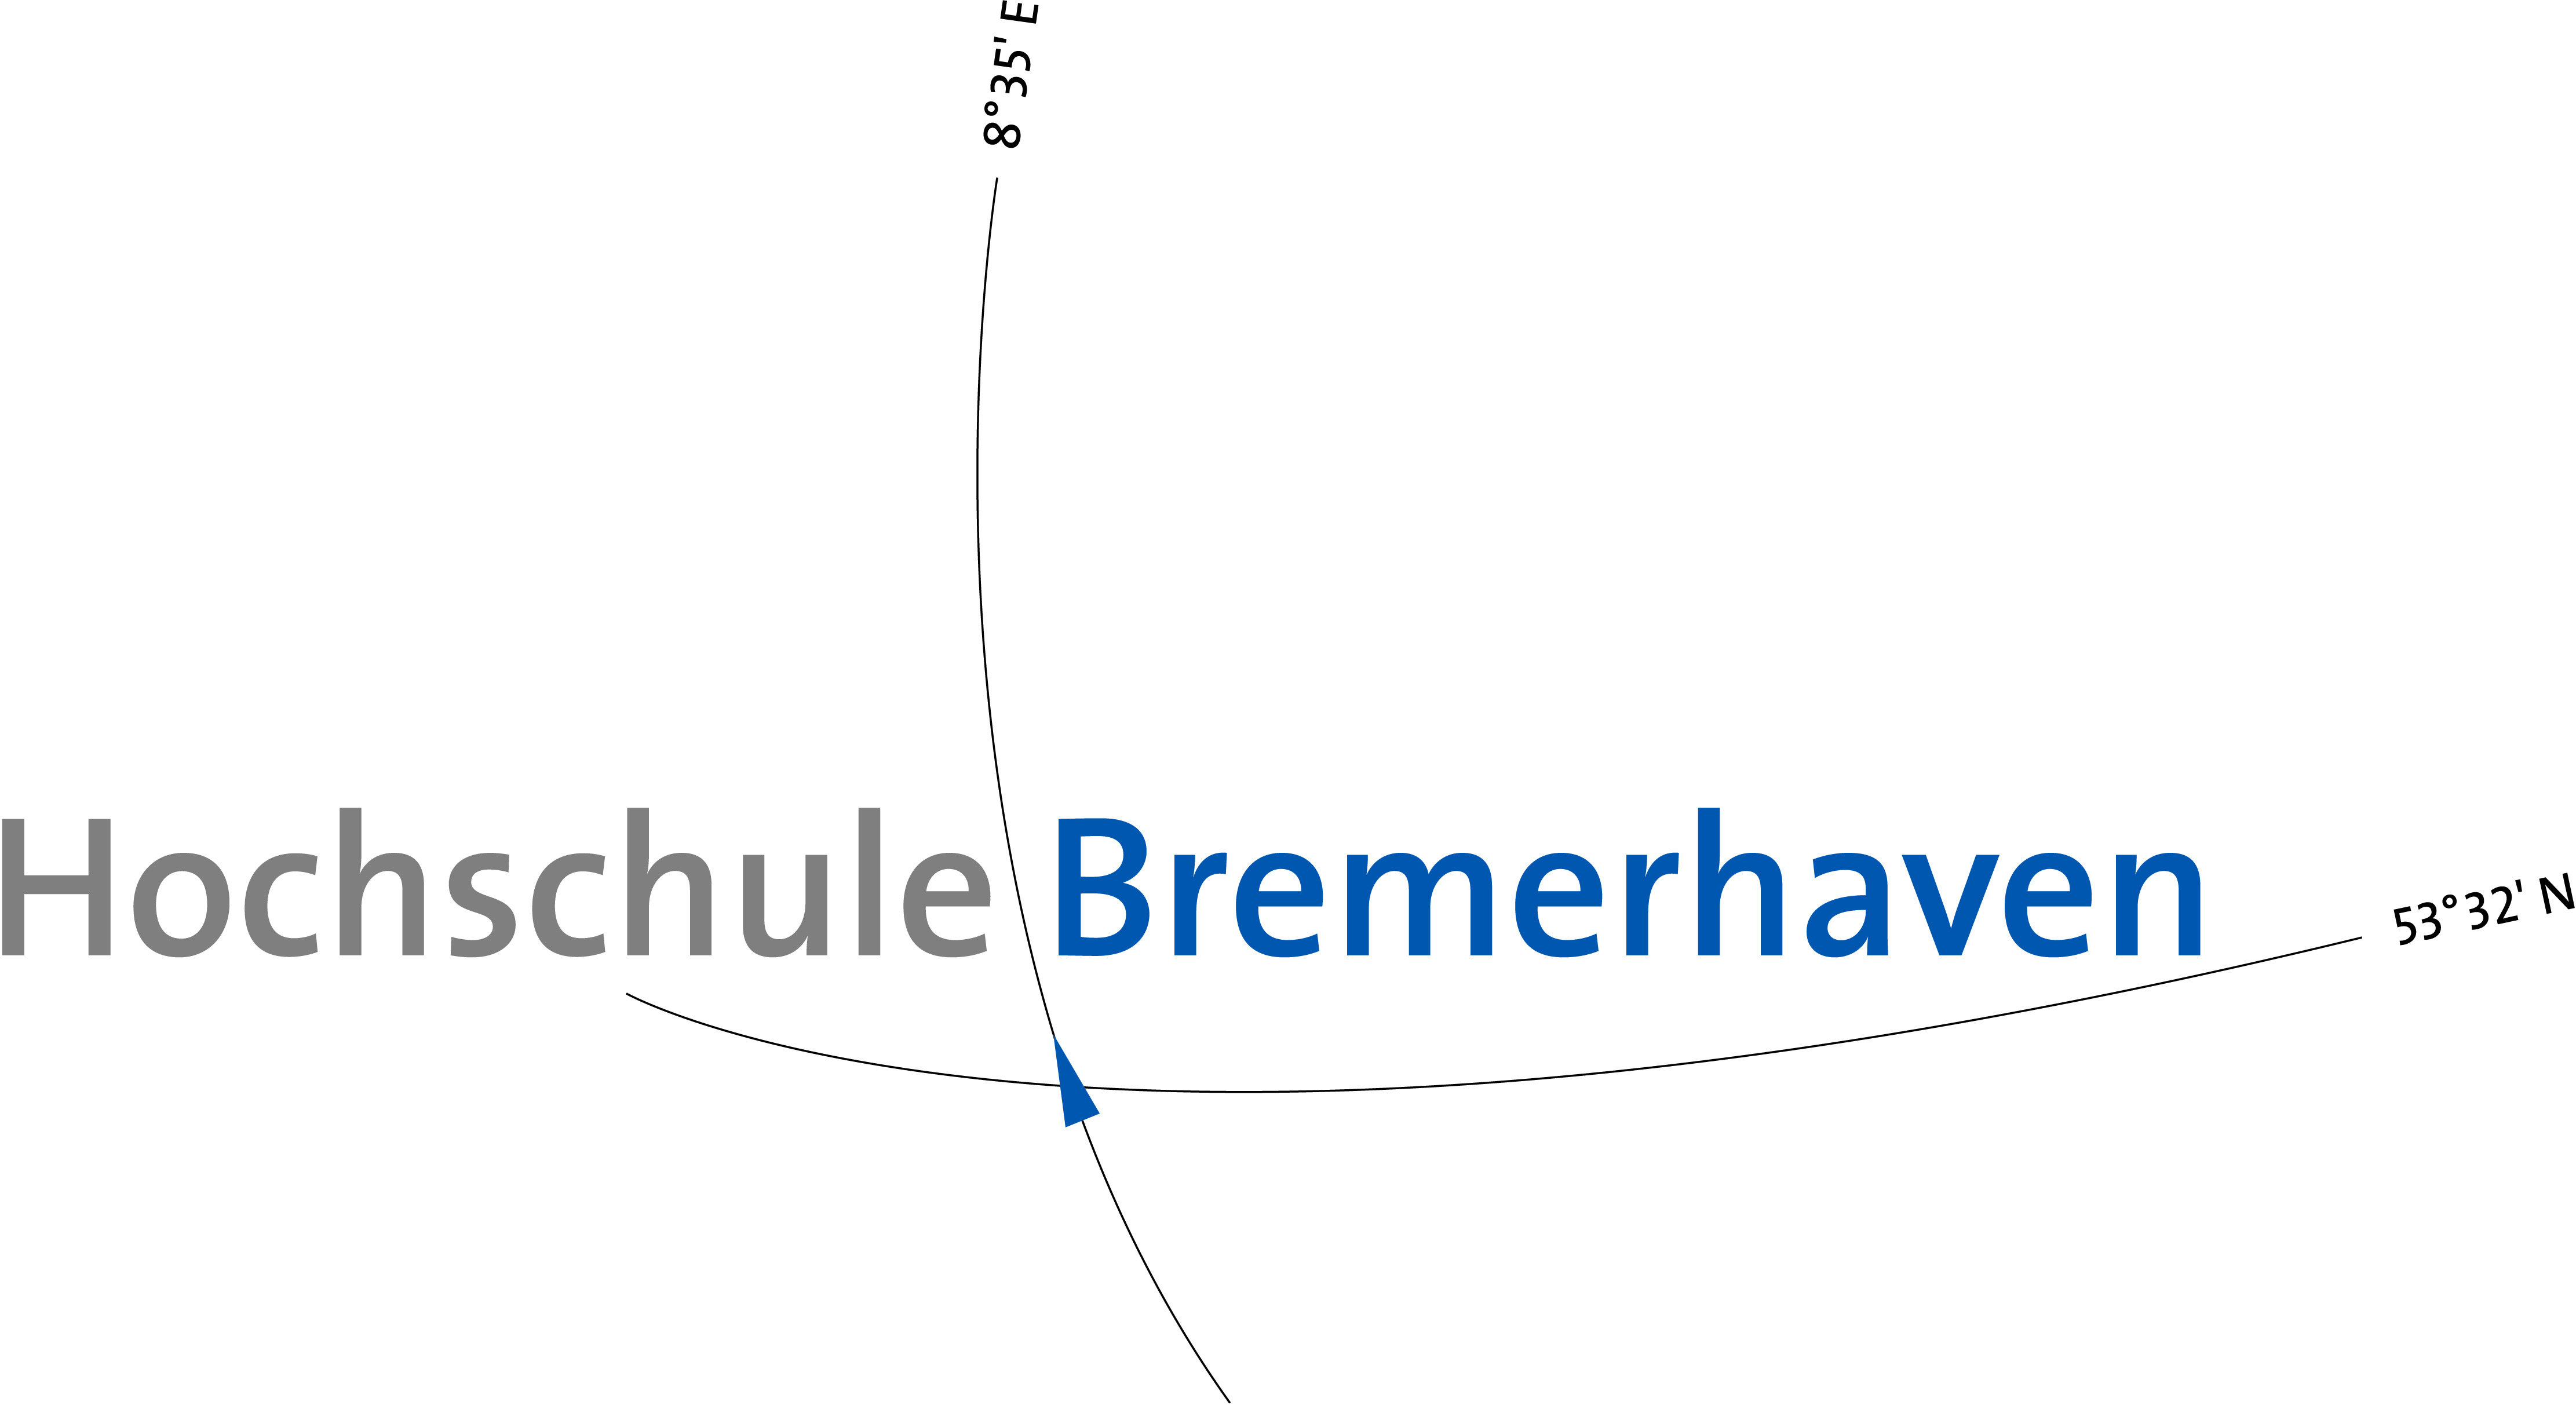
\includegraphics[width=\textwidth]{images/hb_logo_2c.jpg}
        \captionof{figure}{rechts}
        \label{fig:hslogoRight}
      \end{minipage}
\end{figure}
    \subsection{Mathe und Code} \label{sec:mathe}
    \subsubsection*{Mathe}
\begin{equation}\label{eq:successiveReturn}
    \begin{aligned}
    G_t &= R_{t+1} + \gamma R_{t+2} + \gamma^2 R_{t+3} + \gamma^3 R_{t+4} + \dots \\
    &= R_{t+1} + \gamma (R_{t+2} + \gamma R_{t+3} + \gamma^2 R_{t+4} + \dots)  \\
   & = R_{t+1} + \gamma G_{t+1}
    \end{aligned}
\end{equation}

Zu jedem diskreten Zeitpunkt wird dem Agenten eine Belohnung in Form einer einfachen Zahl $R_t \in \mathbb{R}$ zugestellt.

\begin{equation}\label{eq:greedyProbs}
    \pi(a|S_t) =   
        \begin{cases}
            1-\epsilon + \epsilon / |\mathcal{A}(S_t)|      & \quad \text{wenn } a = A_* \\
            \epsilon / |\mathcal{A}(S_t)|  & \quad \text{wenn } a \neq A_*
        \end{cases}
\end{equation}

\begin{equation}\label{eq:wahrscheinlichkeitsverteilung}
    \forall s \in \mathcal{S}: \forall a \in \mathcal{A}(s):
\sum_{s' \in \mathcal{S}} \sum_{r \in \mathcal{R}} p(s', r \mid s,a) = 1 
\end{equation}

\begin{equation}\label{eq:übergangsfunktion}
p(s',r \mid s,a) \doteq Pr\{S_t=s',R_t=r|S_{t-1}=s,A_{t-1}=a\},
\end{equation}

\begin{equation}\label{eq:valueFunction}
    v_\pi(s) = \EX_\pi[G_t \mid S_t = s] = \EX_\pi \left[\sum_{k=0}^\infty{\gamma^k R_{t+k+1} \mid S_t = s} \right]
\end{equation}

\begin{equation}\label{eq:targets}
\begin{aligned}
v_\pi &= \EX_\pi\left[G_t \mid S_t = s \right] \\
&= \EX_\pi\left[R_{t+1} + \gamma G_{t+1} \mid S_t = s \right] \\
        &= \EX_\pi\left[R_{t+1} + \gamma v_\pi(S_{t+1}) \mid S_t = s \right]
\end{aligned}
\end{equation}

\begin{equation}
    B_{2} =  \begin{bmatrix} 
        FOOD\_DROP\_DOWN\_SUCCESS = +1\\
        DEFAULT\_REWARD = -1          
 \end{bmatrix}
\end{equation}



\begin{algorithm}
    \caption{On-policy first-visit MC control (for $\epsilon$-soft policies), estimates $\pi \approx \pi_*$}
    \begin{algorithmic}[1]
        \State Algorithm parameter: small $\epsilon > 0$
        \State Initialize:
        \Indent
           \State $\pi \gets$ an arbitary $\epsilon$-soft policy
           \State $Q(s,a) \in \mathbb{R}$ (arbitrarily), for all $s \in \mathcal{S}, a \in \mathcal{A}(s)$
           \State $Returns(s,a) \gets$ empty list, for all $s \in \mathcal{S}, a \in \mathcal{A}(s)$
        \EndIndent
        \State Repeat forever (for each episode):
        \Indent
            \State Generate an episode following $\pi: S_0, A_0, R_1, \dots, S_{T-1}, A_{T-1}, R_T$
            \State $G \gets 0$
            \State Loop for each step of episode, $t= T-1,T-2, \dots, 0:$
            \Indent
                \State $G \gets \gamma G + R_{t+1}$
                \State Unless the pair $S_t, A_t$ appears in $S_0, A_0, S_1, A_1, \dots ,S_{t-1}, A_{t-1}:$
                \Indent
                    \State Append $G$ to $Returns(S_t,A_t)$
                    \State $Q(S_t,A_t) \gets$ average$(Returns(S_t,A_t))$
                    \State $A^* \gets \argmax_a Q(S_t, a)$ (with ties broken arbitrarily)
                    \State For all $a \in \mathcal{A}(S_t):$
                    \Indent
                     \State  $\pi(a|S_t) =   
                        \begin{cases}
                            1-\epsilon + \epsilon / |\mathcal{A}(S_t)|      & \quad \text{if } a = A^* \\
                            \epsilon / |\mathcal{A}(S_t)|  & \quad \text{if } a \neq A^*
                        \end{cases}$
                    \EndIndent
                \EndIndent
            \EndIndent
        \EndIndent 
    \end{algorithmic}
\end{algorithm}


\begin{lstlisting}[language=json,firstnumber=1, label=lst:ursprüngliche Wahrnehmung,caption=Wahrnehmung des Agenten bei dem ursprünglichen Problem]
{
    "state": "ALIVE",
    "currentFood": 0,
    "totalFood": 0,
    "cell": {
        "row": 0,
        "col": 10,
        "type": "START",
        "food": 0,
        "smell": 0,
        "stench": 0
    }
}}
\end{lstlisting}
    \subsection{Sonstiges} \label{sec:sonstiges}
    Absätze werden mit 
\begin{verbatim}
\par 
\end{verbatim}
gekennzeichnet.
\par
Zwischenüberschriften mit Absatz (der * bedeutet, dass diese subsection nicht im Inhaltsverzeichnis aufgeführt wird:
\subsection*{REST}
Lorem ipsum dolor sit amet, consetetur sadipscing elitr, sed diam nonumy eirmod tempor invidunt ut labore et dolore magna aliquyam erat, sed diam voluptua. At vero eos et accusam et justo duo dolores et ea rebum. Stet clita kasd gubergren, no sea takimata sanctus est Lorem ipsum dolor sit amet.

\par 
Unterpunkte mit hervorgehobenen ersten Wort:
\paragraph{Http} 
Lorem ipsum dolor sit amet, consetetur sadipscing elitr, sed diam nonumy eirmod tempor invidunt ut labore et dolore magna aliquyam erat, sed diam voluptua. At vero eos et accusam et justo duo dolores et ea rebum. Stet clita kasd gubergren, no sea takimata sanctus est Lorem ipsum dolor sit amet.
\newpage
\section{Fazit}
Conclusions.

\newpage
\bibliographystyle{apacite}
\bibliography{sources}
\pagebreak

\end{document}

